\pagebreak
\chapter{METODOLOGI}

Pada bab ini akan dijelaskan langkah-langkah pelaksanaan penelitian tugas akhir yang dilengkapi dengan alur proses serta jadwal kegiatan yang disusun selama penelitian.
% \section{Studi Literatur}
% Pada tahap ini dilakukan pengumpulan referensi yang relevan dengan penelitian tugas akhir ini. Sumber referensi yang digunakan adalah buku, tugas akhir, tesis, paper, serta artikel yang mendukung topik penelitian. Referensi yang terkait dengan penelitian ini adalah mengenai kendali rudal menggunakan metode NMPC dengan pendekatan fungsi laguerre.

\section{Pengkajian Model Matematika Rudal}

\section{Pendiskritan Model}

\section{Pembentukan Kendali Rudal Menggunakan Laguerre-NMPC}

\section{Simulasi dan Analisis Hasil Simulasi}

\section{Penarikan Kesimpulan dan Saran}

\section{Penulisan Laporan Tugas Akhir}

\begin{figure}[htbp]
    \centering
    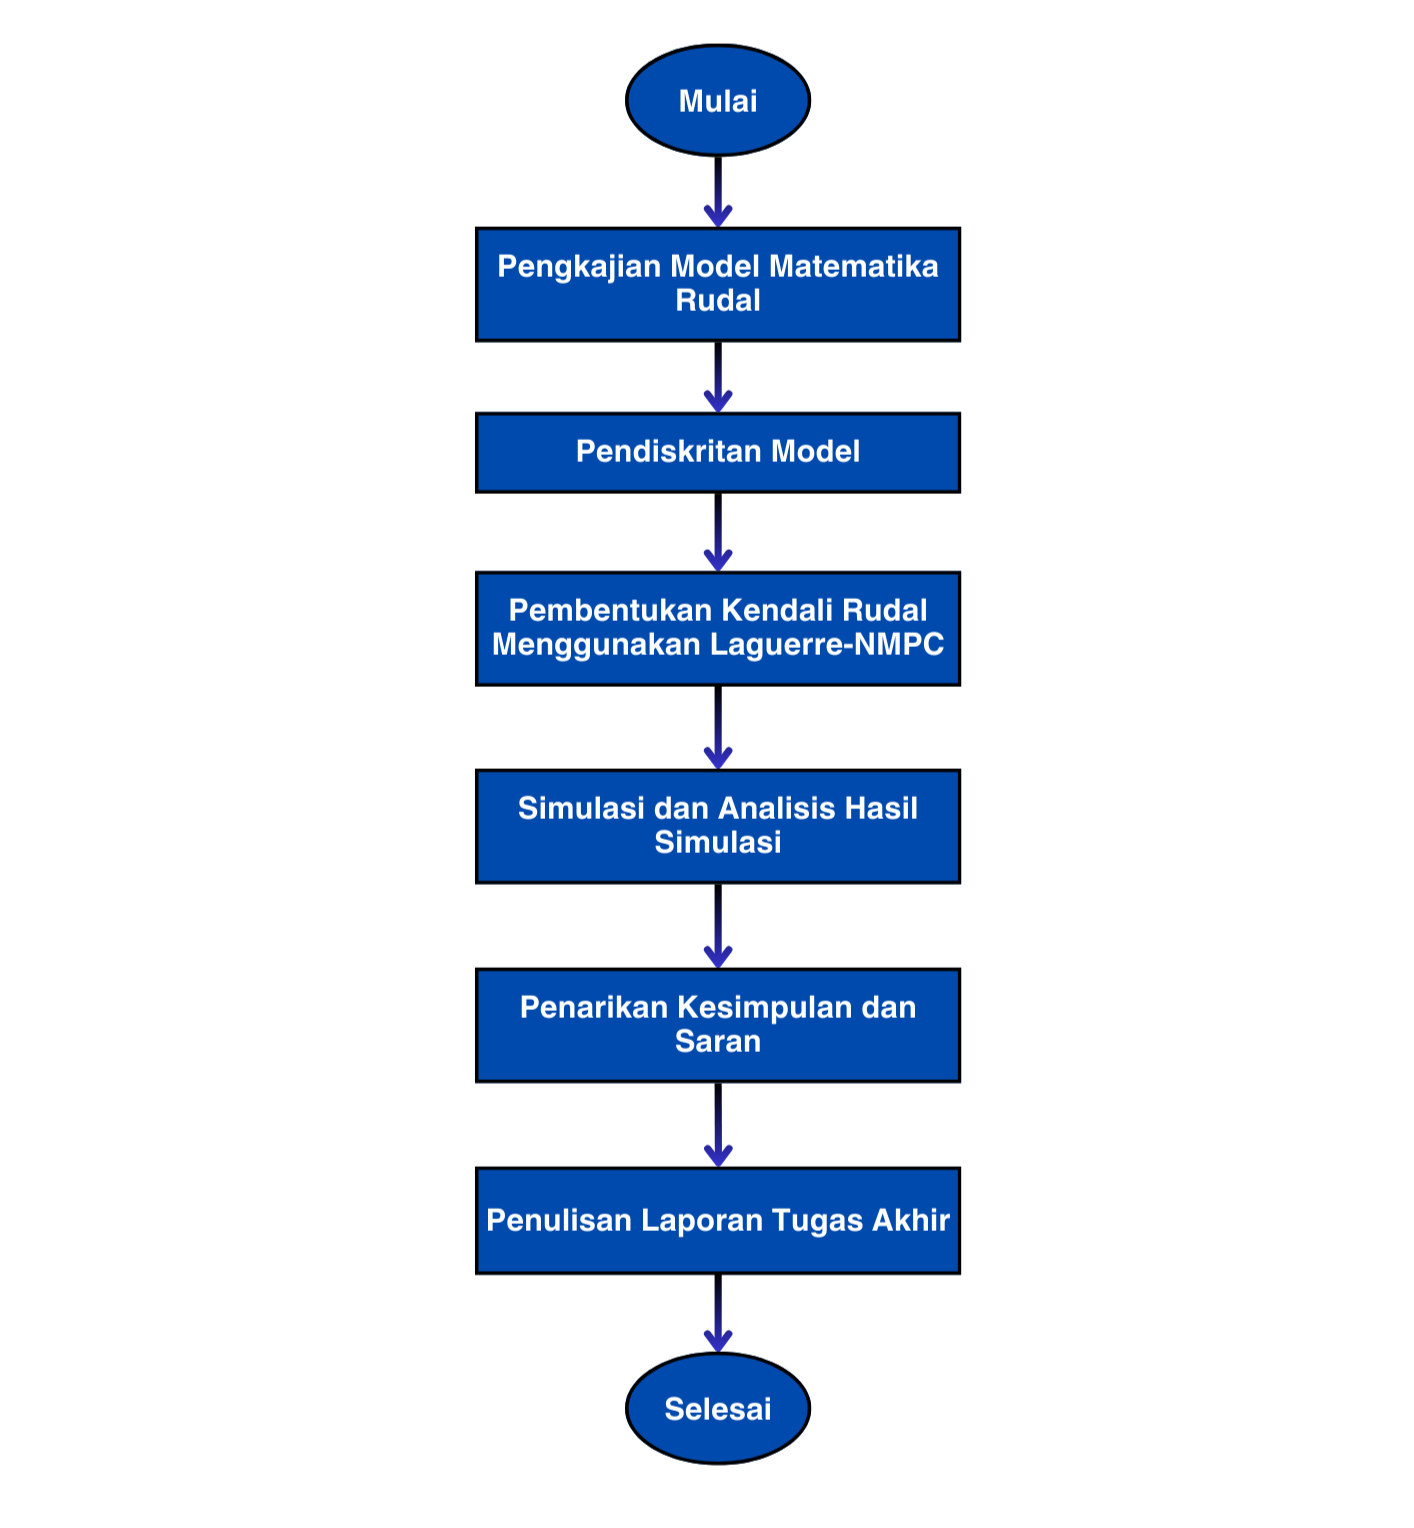
\includegraphics[width=\linewidth]{foto/Diagram Alir Penelitian Blue.png}
    \caption{Diagram Alir Penelitian}
    \label{fig:diagram penelitian}
\end{figure}

\pagebreak
\chapter*{JADWAL PENELITIAN}
Berikut jadwal pelaksanaan tahap-tahap penelitian tugas akhir yang akan dilakukan selama 3 bulan sesuai dengan metode penelitian. \vspace{0.5cm}
\begin{table}[htbp]
\centering
\caption{Jadwal Pelaksanaan Penelitian Tugas Akhir}
\renewcommand{\arraystretch}{1.5}
\begin{tabular}{|C{0.6cm}|L{6.5cm}|C{0.25cm}|C{0.25cm}|C{0.25cm}|C{0.25cm}|C{0.25cm}|C{0.25cm}|C{0.25cm}|C{0.25cm}|C{0.25cm}|C{0.25cm}|C{0.25cm}|C{0.25cm}|}	\hline
	&&\multicolumn{12}{c|}{\textbf{BULAN}}\\\cline{3-14}
	\multicolumn{1}{|c|}{\textbf{NO}}&\multicolumn{1}{c|}{\textbf{NAMA KEGIATAN}}&\multicolumn{4}{c|}{1}&\multicolumn{4}{c|}{2}&\multicolumn{4}{c|}{3}\\\cline{3-14}
	&&1&2&3&4&1&2&3&4&1&2&3&4\\\cline{1-14}
	1&Pengkajian model matematika rudal &\cellcolor{blue!}&\cellcolor{blue!}&&&&&&&&&&\\\hline
	2&Pendiskritan model&&\cellcolor{blue!}&\cellcolor{blue!}&&&&&&&&&\\\hline
	3&Pembentukan kendali rudal menggunakan Laguerre-NMPC &&&\cellcolor{blue!}&\cellcolor{blue!}&&&&&&&&\\\hline
	4&Pembuatan program menggunakan software MATLAB R2024b &&&&\cellcolor{blue!}&\cellcolor{blue!}&\cellcolor{blue!}&\cellcolor{blue!}&&&&&\\\hline
	5&Simulasi dan analisis hasil simulasi&&&&&&&\cellcolor{blue!}&\cellcolor{blue!}&\cellcolor{blue!}&&&\\\hline
	6&Penarikan kesimpulan dan saran&&&&&&&&&\cellcolor{blue!}&\cellcolor{blue!}&&\\\hline
	7&Penulisan laporan tugas akhir&&&&&&&&&&\cellcolor{blue!}&\cellcolor{blue!}&\cellcolor{blue!}\\\hline
\end{tabular}
\end{table}
